\documentclass{beamer}

\mode<presentation> {
}

\title[]{Bayesian Clinical Trials} 
\subtitle{Case study } 
\date{} 

\usepackage{graphicx} 
\usepackage{booktabs} 
\usepackage{longtable} 
 \usepackage{hyperref}


\usepackage{color}
\usepackage{fancyvrb}

\definecolor{shadecolor}{gray}{0.95}

\DefineShortVerb[commandchars=\\\{\}]{\|}
\DefineVerbatimEnvironment{Highlighting}{Verbatim}{commandchars=\\\{\}}
\newenvironment{Shaded}{}{}
\newcommand{\KeywordTok}[1]{\textcolor[rgb]{0.00,0.44,0.13}{\textbf{{#1}}}}
\newcommand{\DataTypeTok}[1]{\textcolor[rgb]{0.56,0.13,0.00}{{#1}}}
\newcommand{\DecValTok}[1]{\textcolor[rgb]{0.25,0.63,0.44}{{#1}}}
\newcommand{\BaseNTok}[1]{\textcolor[rgb]{0.25,0.63,0.44}{{#1}}}
\newcommand{\FloatTok}[1]{\textcolor[rgb]{0.25,0.63,0.44}{{#1}}}
\newcommand{\CharTok}[1]{\textcolor[rgb]{0.25,0.44,0.63}{{#1}}}
\newcommand{\StringTok}[1]{\textcolor[rgb]{0.25,0.44,0.63}{{#1}}}
\newcommand{\CommentTok}[1]{\textcolor[rgb]{0.38,0.63,0.69}{\textit{{#1}}}}
\newcommand{\OtherTok}[1]{\textcolor[rgb]{0.00,0.44,0.13}{{#1}}}
\newcommand{\AlertTok}[1]{\textcolor[rgb]{1.00,0.00,0.00}{\textbf{{#1}}}}
\newcommand{\FunctionTok}[1]{\textcolor[rgb]{0.02,0.16,0.49}{{#1}}}
\newcommand{\RegionMarkerTok}[1]{{#1}}
\newcommand{\ErrorTok}[1]{\textcolor[rgb]{1.00,0.00,0.00}{\textbf{{#1}}}}
\newcommand{\NormalTok}[1]{{#1}}

\hypersetup{breaklinks=true, pdfborder={0 0 0}}
\setlength{\parindent}{0pt}
\setlength{\parskip}{6pt plus 2pt minus 1pt}
\setlength{\emergencystretch}{3em}  
\setcounter{secnumdepth}{0}
%\EndDefineVerbatimEnvironment{Highlighting}


\begin{document}



\begin{frame}
\titlepage % Print the title page as the first slide
\end{frame}



\begin{frame}{Example}

Osteosarcoma is the most common malignant bone tumor in children and
young adults and prognosis after its recurrence is poor.

There is a need to identify novel effective agents and these agents are
usually evaluated initially in patients with relapsed osteosarcoma.

Consider the design of a controlled phase II B trial to compare two
different treatment, say A and B, with (dichotomized) response measured
according to RECIST criteria as outcome.

What sample size is needed to provide sufficient information to specify
the true difference in response rates to within a total interval width
of 20 percentage points?

\end{frame}

\begin{frame}{Evidence}

\begin{longtable}{lllll}
\toprule
Phase II Study & Treatment & Sample Size & Responses (\%) & 95\%
CI\tabularnewline
\midrule
\endhead
1 & A & 26 & 5 (19) &\tabularnewline
2 & B & 37 & 14 (37) & 22;53\tabularnewline
3 & A & 14 & 4 (28.5) &\tabularnewline
\bottomrule
\end{longtable}

Assume a pooled estimate for Treatment A: \(\frac{9}{40}=22.5\)

Assume an estimate for Treatment B: \(\frac{14}{37}=38.0\)

\end{frame}

\begin{frame}[fragile]{Frequentist Sample size (per group) by \(l\) and
\((1-\alpha)\)}

If we consider not only the estimates but also uncertainty, for example
the upper and lower limit of the 95\% confidence interval, we can get
different sample sizes:

\begin{Shaded}
\begin{Highlighting}[]
\KeywordTok{library}\NormalTok{(SampleSizeProportions)}
\end{Highlighting}
\end{Shaded}

\begin{verbatim}
##                         theta
##               -0.01 	    0.02   0.15     0.3
##---------------------------------------------
## length= 0.2     134      141     159     164
## length= 0.21    122      128     144     149
## length= 0.22    111      116     132     136
## length= 0.24     94       98     111     114
## length= 0.25     86       90     102     105
\end{verbatim}

Which is best?

\end{frame}

\begin{frame}{Priors}

\begin{itemize}
\itemsep1pt\parskip0pt\parsep0pt
\item
  For Treatment A we can assume that 0.225 is the mean of a Beta
  distribution: \(Beta\left(c_{1}=9,d_{1}=31\right)\)
\item
  For Treatment B we can assume that 0.38 is the mean of a Beta
  distribution: \(Beta\left(c_{2}=14,d_{2}=23\right)\)
\end{itemize}

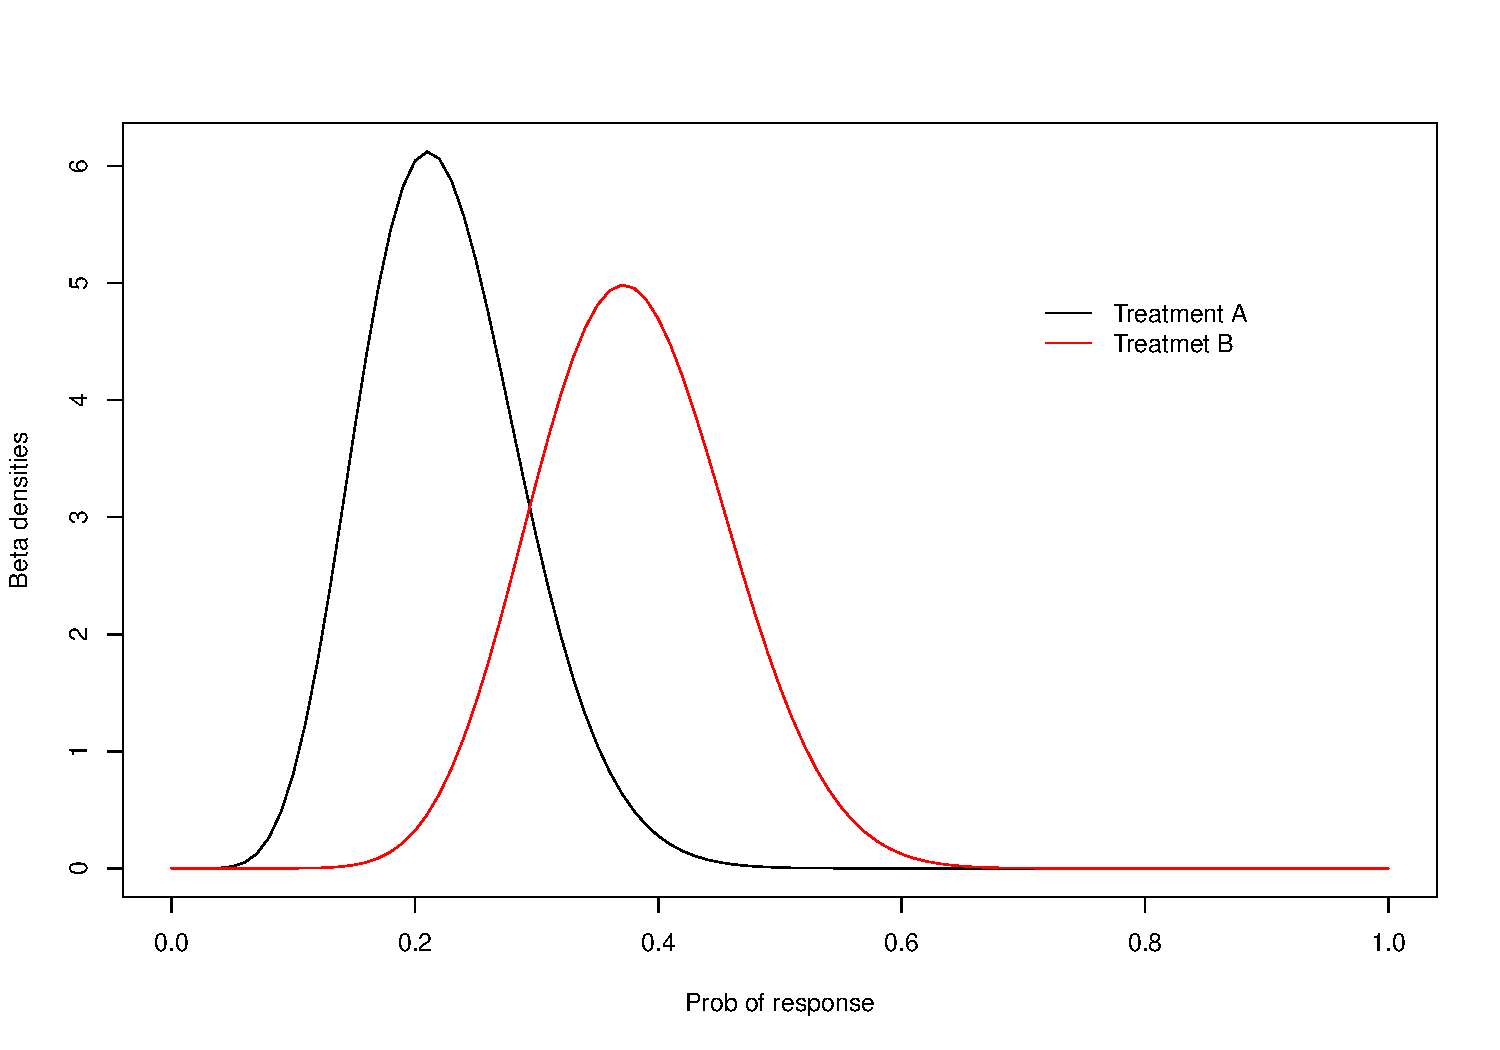
\includegraphics[scale=0.38]{09CaseStudy_files/figure-beamer/unnamed-chunk-3-1.pdf}

\end{frame}

\begin{frame}[fragile]{SampleSizeProportions package}

SampleSizeProportions implements a set of functions for calculating
required sample sizes for

\begin{itemize}
\itemsep1pt\parskip0pt\parsep0pt
\item
  Average Length Criterion (ALC)
\item
  Average Coverage Criterion (ACC)
\item
  Worst Outcome Criterion (WOC)
\end{itemize}

in the context of binomial observations.

\begin{Shaded}
\begin{Highlighting}[]
\KeywordTok{library}\NormalTok{(SampleSizeProportions)}
\end{Highlighting}
\end{Shaded}

\end{frame}

\begin{frame}[fragile]{Bayesian Sample size (per group) by \(l\) and
\((1-\alpha)\)}

\begin{verbatim}
##              lev= 0.9 lev= 0.95 lev= 0.99
##              ACC      ACC       ACC      
## length= 0.2  70       116       229      
## length= 0.22 51       89        182      
## length= 0.25 31       60        132      
##              -        -         -        
##              ALC      ALC       ALC      
## length= 0.2  70       115       225      
## length= 0.22 51       89        180      
## length= 0.25 31       60        130      
##              -        -         -        
##              WOC      WOC       WOC      
## length= 0.2  96       153       292      
## length= 0.22 73       120       234      
## length= 0.25 48       84        172
\end{verbatim}

\end{frame}

\end{document}